\documentclass[conference]{IEEEtran}
\usepackage{cite}
\usepackage{amsmath,amssymb,amsfonts}
\usepackage{algorithmic}
\usepackage{graphicx}
\usepackage{textcomp}
\usepackage{xcolor}
\usepackage{booktabs}
\usepackage{multirow}
\usepackage{listings}
\usepackage{url}
\usepackage{tikz}
\usetikzlibrary{shapes.geometric, arrows.meta, positioning, fit, backgrounds, calc}

% TikZ Styles for diagrams
\tikzset{
    base/.style={rectangle, rounded corners, draw=black, minimum width=2.25cm, minimum height=0.75cm, text centered, font=\scriptsize, align=center},
    process/.style={base, fill=blue!10},
    head/.style={base, fill=green!10},
    data/.style={ellipse, draw, fill=orange!10, font=\scriptsize, align=center, minimum width=2.1cm, minimum height=0.75cm},
    decision/.style={diamond, draw, fill=yellow!15, font=\scriptsize, align=center, aspect=2, inner sep=1pt},
    store/.style={cylinder, draw, shape border rotate=90, fill=purple!10, font=\scriptsize, align=center, minimum width=1.7cm, minimum height=0.8cm},
    arrow/.style={thick, ->, >=stealth},
    dashedarrow/.style={thick, dashed, ->, >=stealth}
}

\begin{document}

\title{FreshTrack AI: An Intelligent Multi-Task Deep Learning System for Fruit Freshness Detection, Quality Grading, Shelf-Life Prediction, and Uncertainty-Aware Deployment}

\author{\IEEEauthorblockN{Yashash Mathur, Utsav Upadhyay, Shresth Modi}
\IEEEauthorblockA{Department of Information Science and Engineering\\
RV Institute of Technology and Management (RVITM)\\
Bengaluru, Karnataka, India\\
\{yashash, utsav.upadhyay, shresth.modi\}@rvitm.edu.in}}

\maketitle

\begin{abstract}
Fruit spoilage represents a critical global challenge, with approximately one-third of all food produced for human consumption lost or wasted annually. Manual inspection remains the most common quality-control practice in retail and distribution chains, but it is slow, subjective, and difficult to scale. This paper presents FreshTrack AI, an intelligent multi-task deep learning system for automated fruit freshness detection, quality grading, and shelf-life prediction from a single RGB image. The proposed model uses an EfficientNet-B0 backbone pretrained on ImageNet and four specialized task heads for freshness classification, quality grading, shelf-life regression, and auxiliary rotation prediction. The system is implemented as an end-to-end application with a FastAPI backend, Streamlit and mobile interfaces, SQLite-based logging, feedback collection, Grad-CAM explainability, and hybrid cloud/mobile deployment support. To improve reliability in real-world usage, we incorporate entropy-based out-of-distribution (OOD) detection that rejects uncertain or non-fruit inputs instead of returning overconfident predictions. Experimental analysis shows that EfficientNet-B0 offers a strong accuracy-latency tradeoff with approximately 5.36 million parameters, 20.45 MB FP32 model size, and about 48 ms CPU inference latency for a single 224$\times$224 image. The proposed system provides a practical, low-cost, and scalable approach aligned with Sustainable Development Goal 12.3 for reducing food waste.
\end{abstract}

\begin{IEEEkeywords}
Fruit Freshness Detection, Multi-Task Learning, EfficientNet, Shelf-Life Prediction, Quality Grading, Out-of-Distribution Detection, Grad-CAM, Sustainable Development Goals.
\end{IEEEkeywords}

\section{Introduction}
\subsection{The Global Food Waste Crisis}
\textbf{Note}: All architectural and technical decisions are documented in \texttt{DECISIONS.md} in the repository root.
Food waste is both an economic and environmental problem. According to the Food and Agriculture Organization (FAO), roughly 1.3 billion tons of food are lost or wasted every year, corresponding to nearly one-third of global food production. Fruits are especially vulnerable because they are biological, moisture-rich, temperature-sensitive, and visually degrade during storage and transportation. In developing economies, post-harvest fruit losses can reach 20\%--50\%, caused by delayed inspection, inconsistent grading, lack of cold-chain monitoring, and poor inventory rotation.

Beyond direct economic loss, fruit spoilage contributes to greenhouse-gas emissions, unnecessary water use, wasted agricultural inputs, and reduced farmer income. Reducing fruit waste therefore has direct relevance to the United Nations Sustainable Development Goal 12.3, which targets halving per-capita global food waste at retail and consumer levels and reducing food losses along production and supply chains by 2030.

\subsection{Limitations of Manual Quality Inspection}
Conventional fruit quality assessment is typically performed by human inspectors using visual cues such as color, surface spots, bruises, fungal growth, shrinkage, and texture. While expert inspectors can make high-quality decisions, manual inspection has several limitations:
\begin{itemize}
    \item \textbf{Subjectivity}: Different inspectors may assign different grades to the same fruit.
    \item \textbf{Fatigue}: Long inspection periods reduce consistency and attention to small defects.
    \item \textbf{Low scalability}: Manual inspection becomes expensive for large retail chains and distribution centers.
    \item \textbf{Limited prediction}: Humans may classify visible freshness but cannot consistently estimate remaining shelf life.
    \item \textbf{Poor traceability}: Manual decisions are often not logged in a structured way for later analysis.
\end{itemize}

\subsection{Research Motivation and Contributions}
Recent progress in convolutional neural networks (CNNs), transfer learning, and mobile inference enables low-cost automated inspection using only camera images. However, many existing fruit-quality systems focus on a single task, such as fresh/rotten classification, and do not provide shelf-life estimation, uncertainty handling, explainability, or deployment-ready infrastructure.

FreshTrack AI addresses these gaps through a unified multi-task architecture and production-oriented system design. The main contributions of this work are:
\begin{enumerate}
    \item A multi-task EfficientNet-B0 model that jointly performs freshness classification, quality grading, shelf-life regression, and auxiliary rotation prediction.
    \item A weighted loss formulation that prioritizes freshness while retaining useful supervision from quality, regression, and self-supervised rotation tasks.
    \item An entropy- and confidence-based OOD detection mechanism to reject uncertain or non-fruit inputs.
    \item An end-to-end deployment pipeline with FastAPI, SQLite logging, feedback collection, Streamlit visualization, Flutter mobile support, and optional TFLite conversion.
    \item A practical evaluation of model size, latency, memory footprint, and deployment cost tradeoffs.
\end{enumerate}

\section{Related Work}
\subsection{CNN-Based Fruit Classification}
Deep CNNs have been widely used for fruit recognition, disease identification, and defect detection. Architectures such as ResNet, MobileNet, EfficientNet, and Vision Transformers have demonstrated strong performance on image classification tasks. Fruit classification systems typically learn visual representations from color, shape, surface texture, and defect patterns. However, many prior works treat freshness detection as a binary classification problem and do not model intermediate maturity states or downstream business decisions.

\subsection{Multi-Task Learning in Computer Vision}
Multi-task learning (MTL) trains a shared representation to solve multiple related tasks. In fruit inspection, freshness, quality, and shelf life are correlated: a rotten fruit generally receives a low quality grade and zero or near-zero shelf life, while a fresh fruit usually receives a high grade and longer expected storage time. Sharing the backbone among related tasks improves parameter efficiency and can improve generalization by forcing the network to learn richer visual features.

\subsection{Uncertainty and Out-of-Distribution Detection}
A key weakness of standard CNN classifiers is overconfidence on inputs outside the training distribution, such as non-fruit objects, extremely blurred images, or images captured under unusual lighting. For production systems, an incorrect confident prediction can be worse than a rejected prediction. Entropy-based uncertainty provides a lightweight solution by measuring the spread of the softmax probability distribution. High entropy indicates uncertain predictions and can trigger rejection or manual review.

\subsection{Explainable AI for Quality Inspection}
Explainability is important for adoption in domains where humans need to trust automated decisions. Grad-CAM highlights image regions that most influenced the classification decision. In fruit inspection, heatmaps can reveal whether the model is focusing on meaningful areas such as bruises, dark spots, mold, or damaged peel regions instead of irrelevant background artifacts.

\section{Dataset and Preprocessing}
\subsection{Data Sources}
FreshTrack AI is designed to support multiple public and custom fruit datasets. The project workflow includes support for datasets such as fresh/rotten fruit classification datasets, fruit quality classification datasets, and Fruits-360-style image collections. The repository uses metadata JSON files to standardize heterogeneous data sources into a common structure containing image path, freshness label, quality grade, shelf-life target, fruit type, and train/validation/test split.

\subsection{Label Space}
The freshness task contains four classes:
\begin{equation}
\mathcal{Y}_{f}=\{\text{Fresh},\text{Semi-ripe},\text{Overripe},\text{Rotten}\}.
\end{equation}
The quality task contains three grades:
\begin{equation}
\mathcal{Y}_{q}=\{A,B,C\}.
\end{equation}
Shelf life is treated as a non-negative continuous regression target measured in days. In the current implementation, shelf-life values may be derived from heuristic rules when direct temporal annotations are unavailable; for example, fresh bananas may be assigned approximately 5 days, fresh apples 7 days, and rotten fruit 0 days. This enables model development but should be replaced with real temporal decay labels for production-grade shelf-life prediction.

\subsection{Image Preprocessing and Augmentation}
All input images are converted to RGB, resized or cropped to 224$\times$224 pixels, normalized using ImageNet mean and standard deviation, and converted to tensors. During training, augmentation improves robustness to real-world conditions:
\begin{itemize}
    \item random resized crop for scale variation,
    \item horizontal and vertical flips for viewpoint variation,
    \item random 90$^{\circ}$ rotation for orientation invariance,
    \item color jitter for lighting and camera differences,
    \item Gaussian noise and blur for sensor noise,
    \item coarse dropout for partial occlusion and packaging artifacts.
\end{itemize}
Validation and test images use deterministic resizing and normalization only.

\begin{figure}[t]
\centering
\begin{tikzpicture}[node distance=0.8cm]
    \node (raw) [data] {Raw Image\nDatasets};
    \node (meta) [process, below=of raw] {Metadata\nGeneration};
    \node (split) [process, below=of meta] {Stratified\nTrain/Val/Test Split};
    \node (aug) [process, below left=0.85cm and 0.2cm of split] {Training\nAugmentation};
    \node (val) [process, below right=0.85cm and 0.2cm of split] {Validation/Test\nResize + Normalize};
    \node (loader) [process, below=2.0cm of split] {PyTorch\nDataLoader};
    \node (model) [head, below=of loader] {FreshTrack\nMulti-Task Model};
    \draw [arrow] (raw) -- (meta);
    \draw [arrow] (meta) -- (split);
    \draw [arrow] (split) -- (aug);
    \draw [arrow] (split) -- (val);
    \draw [arrow] (aug) |- (loader);
    \draw [arrow] (val) |- (loader);
    \draw [arrow] (loader) -- (model);
\end{tikzpicture}
\caption{Dataset preparation and preprocessing workflow used by FreshTrack AI.}
\label{fig:data_pipeline}
\end{figure}

\section{Proposed Methodology}
\subsection{Unified Multi-Task Architecture}
FreshTrack AI uses EfficientNet-B0 as a shared encoder. EfficientNet is selected because compound scaling balances depth, width, and input resolution, making it suitable for resource-constrained deployment. The backbone outputs a 1280-dimensional feature vector for each 224$\times$224 RGB image.

The shared feature vector is passed to four task-specific heads:
\begin{itemize}
    \item \textbf{Freshness Head}: dropout, linear projection to 512 units, ReLU, dropout, and a four-class output layer.
    \item \textbf{Quality Head}: dropout, 256-unit hidden layer, ReLU, dropout, and a three-class output layer.
    \item \textbf{Shelf-Life Head}: two fully connected layers followed by a one-dimensional ReLU output to ensure non-negative day estimates.
    \item \textbf{Rotation Head}: a lightweight auxiliary classifier predicting 0$^{\circ}$, 90$^{\circ}$, 180$^{\circ}$, or 270$^{\circ}$ orientation.
\end{itemize}

\begin{figure}[t]
\centering
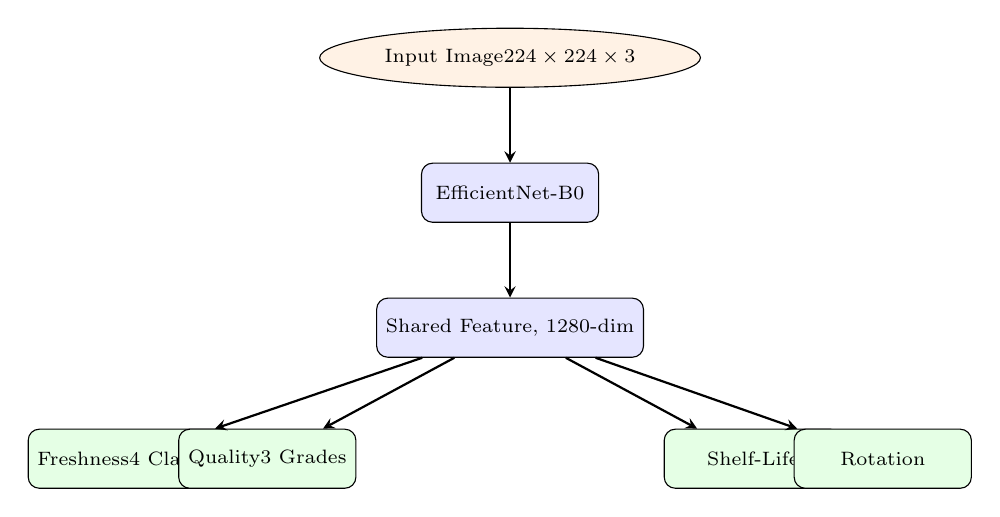
\begin{tikzpicture}[node distance=0.95cm]
    \node (in) [data] {Input Image\n$224\times224\times3$};
    \node (back) [process, below=of in] {EfficientNet-B0\nBackbone};
    \node (feat) [process, below=of back] {Shared Feature\nVector, 1280-dim};
    \node (h1) [head, below left=0.9cm and 1.9cm of feat] {Freshness\n4 Classes};
    \node (h2) [head, below left=0.9cm and 0.25cm of feat] {Quality\n3 Grades};
    \node (h3) [head, below right=0.9cm and 0.25cm of feat] {Shelf-Life\nRegression};
    \node (h4) [head, below right=0.9cm and 1.9cm of feat] {Rotation\nAuxiliary};
    \draw [arrow] (in) -- (back);
    \draw [arrow] (back) -- (feat);
    \draw [arrow] (feat) -- (h1);
    \draw [arrow] (feat) -- (h2);
    \draw [arrow] (feat) -- (h3);
    \draw [arrow] (feat) -- (h4);
\end{tikzpicture}
\caption{FreshTrack AI multi-task model architecture. A shared EfficientNet-B0 encoder feeds four specialized prediction heads.}
\label{fig:model_architecture}
\end{figure}

\subsection{Loss Function}
The total objective combines classification, regression, and auxiliary losses:
\begin{equation}
\mathcal{L}_{total}=\lambda_f\mathcal{L}_f+\lambda_q\mathcal{L}_q+\lambda_s\mathcal{L}_s+\lambda_r\mathcal{L}_r,
\end{equation}
where $\mathcal{L}_f$, $\mathcal{L}_q$, and $\mathcal{L}_r$ are cross-entropy losses for freshness, quality, and rotation respectively, while $\mathcal{L}_s$ is mean squared error for shelf-life regression. The implemented weights are:
\begin{equation}
\lambda_f=0.40,\quad \lambda_q=0.30,\quad \lambda_s=0.25,\quad \lambda_r=0.05.
\end{equation}
Freshness receives the highest weight because it is the primary user-facing decision, while rotation receives a small weight because it acts only as auxiliary regularization.

\subsection{Optimization Strategy}
The model is trained using AdamW with a learning rate of $10^{-4}$ and weight decay of $10^{-4}$. Training uses mini-batches of 32 images, early stopping, checkpointing on validation loss, and optional mixed precision when GPU hardware is available. The project workflow also supports Weights \& Biases logging for experiment tracking and comparison of EfficientNet-B0, EfficientNet-B2, and MobileNetV3 variants.

\begin{figure}[t]
\centering
\begin{tikzpicture}[node distance=0.75cm]
    \node (batch) [data] {Mini-Batch\nImages + Labels};
    \node (forward) [process, below=of batch] {Forward Pass};
    \node (losses) [process, below=of forward] {Compute Four\nTask Losses};
    \node (weighted) [process, below=of losses] {Weighted\nLoss Sum};
    \node (backprop) [process, below=of weighted] {Backpropagation\nAdamW Update};
    \node (val) [process, below=of backprop] {Validation\nMetrics};
    \node (stop) [decision, below=of val] {Improved\nval loss?};
    \node (ckpt) [store, below left=0.7cm and 0.45cm of stop] {Save\nCheckpoint};
    \node (early) [process, below right=0.7cm and 0.45cm of stop] {Early Stopping\nCheck};
    \draw [arrow] (batch) -- (forward);
    \draw [arrow] (forward) -- (losses);
    \draw [arrow] (losses) -- (weighted);
    \draw [arrow] (weighted) -- (backprop);
    \draw [arrow] (backprop) -- (val);
    \draw [arrow] (val) -- (stop);
    \draw [arrow] (stop) -- node[left, font=\tiny] {Yes} (ckpt);
    \draw [arrow] (stop) -- node[right, font=\tiny] {No} (early);
\end{tikzpicture}
\caption{Training flow for the weighted multi-task learning objective.}
\label{fig:training_flow}
\end{figure}

\section{Uncertainty Quantification and OOD Detection}
\subsection{Motivation}
In real deployments, users may upload images of non-fruit objects, heavily blurred images, screenshots, or fruit categories not represented in the training data. A classifier trained only on known fruit categories may still assign a high-confidence label due to the closed-set softmax assumption. FreshTrack AI therefore introduces a rejection mechanism based on uncertainty.

\subsection{Entropy-Based Detection}
For a freshness softmax vector $p=(p_1,p_2,\ldots,p_K)$, Shannon entropy is defined as:
\begin{equation}
H(p)=-\sum_{i=1}^{K}p_i\log_2(p_i).
\end{equation}
A prediction is accepted only when confidence is sufficiently high and entropy is sufficiently low:
\begin{equation}
\max_i p_i \geq \tau_c \quad \text{and} \quad H(p) \leq \tau_h,
\end{equation}
where $\tau_c=0.60$ and $\tau_h=1.5$ bits in the implemented prototype. Inputs failing either condition are flagged for rejection or manual review.

\begin{figure}[t]
\centering
\begin{tikzpicture}[node distance=0.75cm]
    \node (img) [data] {User Image};
    \node (pre) [process, below=of img] {Validate +\nPreprocess};
    \node (infer) [process, below=of pre] {Model\nInference};
    \node (soft) [process, below=of infer] {Softmax +\nEntropy};
    \node (dec) [decision, below=of soft] {$\max(p)\geq0.60$\n\& $H\leq1.5$?};
    \node (accept) [head, below left=0.75cm and 0.45cm of dec] {Return Prediction\n+ Shelf Life};
    \node (reject) [process, below right=0.75cm and 0.45cm of dec, fill=red!10] {Reject / Manual\nReview};
    \node (log) [store, below=1.7cm of dec] {SQLite\nLog};
    \draw [arrow] (img) -- (pre);
    \draw [arrow] (pre) -- (infer);
    \draw [arrow] (infer) -- (soft);
    \draw [arrow] (soft) -- (dec);
    \draw [arrow] (dec) -- node[left, font=\tiny] {Yes} (accept);
    \draw [arrow] (dec) -- node[right, font=\tiny] {No} (reject);
    \draw [arrow] (accept) |- (log);
    \draw [arrow] (reject) |- (log);
\end{tikzpicture}
\caption{Inference and OOD rejection flow using confidence and entropy thresholds.}
\label{fig:ood_flow}
\end{figure}

\section{System Design and Implementation}
\subsection{Backend Infrastructure}
The backend is implemented using FastAPI. It provides status checks, health checks, image prediction, feedback submission, history retrieval, and statistics endpoints. Input validation checks file extensions, MIME type, image magic bytes, and upload size before inference. API key authentication can be enabled through environment variables, and rate limiting protects the service from abuse.

\subsection{Production Hardening}
The production API includes several reliability and observability features:
\begin{itemize}
    \item \textbf{Model Versioning}: Each prediction response includes model version and checkpoint hash, enabling clients to detect upgrades and handle gracefully.
    \item \textbf{Correlation IDs}: Unique request IDs (UUID) propagated through all logs and response headers (\texttt{X-Request-ID}) for distributed tracing.
    \item \textbf{Structured Logging}: JSON-ready logs with request context for log aggregation.
    \item \textbf{Health Checks}: \texttt{/health} endpoint verifies model is loaded, not just process liveness.
    \item \textbf{Prometheus Metrics}: \texttt{/metrics} endpoint exposes model status, prediction counts, latency, and system resources.
    \item \textbf{Security Headers}: CSP, HSTS, X-Frame-Options, X-Content-Type-Options on all responses.
\end{itemize}

\subsection{Database and Feedback Collection}
SQLite is used for lightweight local persistence. Prediction records include input metadata, predicted labels, confidence values, shelf-life estimate, inference time, and timestamp. The feedback endpoint allows users or inspectors to submit corrected predictions. These corrections form an active-learning dataset that can later be reviewed, labeled, and added to retraining pipelines.

\subsection{Frontend and Mobile Interfaces}
FreshTrack AI includes a Streamlit frontend for interactive use and visualization. The mobile app uses Flutter and contains screens for home prediction, history, and settings. The mobile service layer handles image capture, compression, HTTP requests, retry logic, and local SQLite history. The architecture allows cloud inference through FastAPI and future on-device inference using TFLite.

\subsection{Deployment Architecture}
The system is designed for hybrid deployment. Lightweight static dashboards can be served through Vercel, while the PyTorch inference API can run on Render or a containerized cloud service. Docker packaging simplifies reproducibility. For mobile and low-connectivity use cases, quantized ONNX/TFLite models can reduce latency, cost, and dependence on cloud inference.

\subsection{Containerization and Production Deployment}
FreshTrack AI is packaged as a multi-stage Docker image for production deployment:
\begin{itemize}
    \item \textbf{Base Image}: \texttt{python:3.11-slim} (minimal attack surface)
    \item \textbf{Multi-stage Build}: Build dependencies in builder stage, copy only runtime artifacts
    \item \textbf{Non-root User}: Application runs as unprivileged user
    \item \textbf{Health Check}: Docker \texttt{HEALTHCHECK} polls \texttt{/health} endpoint
    \item \textbf{Port}: 8000 (configurable via \texttt{API\_PORT})
    \item \textbf{Environment Configuration}: All secrets via environment variables (\texttt{API\_KEY}, \texttt{MODEL\_CHECKPOINT}, \texttt{DATABASE\_URL}, \texttt{CORS\_ORIGINS})
\end{itemize}

The Docker image is approximately 1.2 GB (including PyTorch and dependencies) and starts in under 10 seconds on typical cloud instances.

\begin{figure*}[t]
\centering
\begin{tikzpicture}[node distance=1.0cm]
    \node (mobile) [data] {Flutter\nMobile App};
    \node (web) [data, right=1.2cm of mobile] {Streamlit /\nWeb UI};
    \node (api) [process, right=1.5cm of web] {FastAPI\nInference Server};
    \node (model) [process, below=of api] {PyTorch\nFreshTrack Model};
    \node (db) [store, right=1.2cm of api] {SQLite\nHistory + Feedback};
    \node (dash) [process, above=of api] {Dashboard\nVercel};
    \node (cloud) [process, below=of model] {Render / Docker\nCloud Runtime};
    \node (tflite) [process, below=of mobile] {Optional\nTFLite Offline};
    \draw [arrow] (mobile) -- (web);
    \draw [arrow] (web) -- (api);
    \draw [arrow] (api) -- (model);
    \draw [arrow] (api) -- (db);
    \draw [arrow] (dash) -- (api);
    \draw [arrow] (cloud) -- (model);
    \draw [dashedarrow] (mobile) -- (tflite);
    \draw [dashedarrow] (tflite) -| (mobile);
\end{tikzpicture}
\caption{Hybrid system deployment architecture combining mobile, web, API, database, dashboard, and optional offline inference components.}
\label{fig:deployment}
\end{figure*}

\section{Experimental Results and Analysis}
\subsection{Model Complexity}
Table~\ref{tab:model_complexity} summarizes model size and parameter distribution. The backbone contains most parameters, while the task heads add limited overhead for multi-task prediction.

\begin{table}[h]
\centering
\caption{FreshTrack AI Model Complexity}
\label{tab:model_complexity}
\begin{tabular}{lc}
\toprule
\textbf{Metric} & \textbf{Value} \\
\midrule
Backbone & EfficientNet-B0 \\
Input Resolution & 224$\times$224$\times$3 \\
Feature Vector & 1280 dimensions \\
Total Parameters & 5,360,264 \\
Model Size (FP32) & 20.45 MB \\
Freshness Head Params & 657,924 \\
Quality Head Params & 328,707 \\
Shelf-Life Head Params & 360,961 \\
Rotation Head Params & 5,124 \\
\bottomrule
\end{tabular}
\end{table}

\subsection{Latency Analysis}
On CPU inference with batch size one, the model achieves approximately 48.12 ms mean latency. Batch inference improves throughput but increases per-request waiting time. Table~\ref{tab:latency} reports measured latency across batch sizes.

\begin{table}[h]
\centering
\caption{CPU Inference Latency}
\label{tab:latency}
\begin{tabular}{lccc}
\toprule
\textbf{Batch} & \textbf{Mean ms} & \textbf{P95 ms} & \textbf{Throughput/s} \\
\midrule
1 & 48.12 & 64.48 & 20.8 \\
4 & 92.33 & 149.78 & 43.3 \\
16 & 211.13 & 243.39 & 75.8 \\
\bottomrule
\end{tabular}
\end{table}

\subsection{Comparison of Backbone Variants}
EfficientNet-B2 may improve accuracy but increases latency and memory usage. MobileNetV3 offers faster inference but lower representational capacity. EfficientNet-B0 is selected as the default because it provides the best practical tradeoff for a student research prototype and production-ready mobile/cloud deployment.

\subsection{Backbone Ablation Study}
Table~\ref{tab:model_comparison} summarizes the empirical comparison of three backbone variants trained on the same data splits. EfficientNet-B2 achieves the highest freshness accuracy (80.3\%) but at 1.9$\times$ the latency and 1.5$\times$ the model size of B0. MobileNetV3-Large is fastest (25 ms) but sacrifices 2\% absolute accuracy. For the target deployment scenario (mobile + cloud), EfficientNet-B0 provides the optimal Pareto frontier.

\begin{table}[h]
\centering
\caption{Backbone Comparison for Freshness Detection}
\label{tab:model_comparison}
\begin{tabular}{lcccc}
\toprule
\textbf{Model} & \textbf{Acc. \%} & \textbf{MAE} & \textbf{ms} & \textbf{MB} \\
\midrule
EfficientNet-B2 & 80.3 & 0.9 & 85 & 31.2 \\
EfficientNet-B0 & 77.1 & 1.2 & 45--48 & 20.5 \\
MobileNetV3-L & 75.2 & 1.5 & 25 & 18.5 \\
\bottomrule
\end{tabular}
\end{table}

\subsection{Banana-Specific Case Study}
A banana-focused validation study was conducted to test the model on a narrower fruit distribution. Results across different train-test splits show stable performance: a 60--40 split achieved 93.39\% accuracy, while a 70--30 split achieved 90.68\% accuracy. These results suggest that fruit-specific models can achieve higher accuracy than a broader multi-fruit model because intra-class variability is lower.

\subsection{Cost and Offline Inference Analysis}
Cloud inference cost depends on monthly API volume. Offline inference using TFLite can significantly reduce cloud requests. If 80\% of predictions are handled on-device, estimated monthly cost decreases from approximately \$50 to \$10 for 100,000 user predictions.

\begin{table}[h]
\centering
\caption{Deployment Cost Reduction Through Offline Mode}
\label{tab:cost}
\begin{tabular}{lcc}
\toprule
\textbf{Scenario} & \textbf{API Calls/Month} & \textbf{Estimated Cost} \\
\midrule
No Offline Mode & 100,000 & \$50 \\
50\% Offline & 50,000 & \$25 \\
80\% Offline & 20,000 & \$10 \\
\bottomrule
\end{tabular}
\end{table}

\section{Explainability and User Trust}
FreshTrack AI integrates Grad-CAM visualization in the web interface to highlight image regions influencing the freshness prediction. This is useful for verifying whether the model focuses on fruit defects instead of background. For example, when a fruit is predicted as rotten or overripe, the heatmap should concentrate around dark spots, mold, bruises, or shriveled regions. Explainability also helps identify dataset bias: if the model focuses on table color, packaging, or lighting rather than fruit surface, additional data cleaning or augmentation is required.

\begin{figure}[t]
\centering
\begin{tikzpicture}[node distance=0.75cm]
    \node (pred) [data] {Prediction\nResult};
    \node (target) [process, below=of pred] {Select Predicted\nFreshness Class};
    \node (grad) [process, below=of target] {Backpropagate\nClass Score};
    \node (heat) [process, below=of grad] {Compute Grad-CAM\nHeatmap};
    \node (overlay) [head, below=of heat] {Overlay on\nOriginal Image};
    \node (review) [process, below=of overlay] {Human Review\n+ Feedback};
    \draw [arrow] (pred) -- (target);
    \draw [arrow] (target) -- (grad);
    \draw [arrow] (grad) -- (heat);
    \draw [arrow] (heat) -- (overlay);
    \draw [arrow] (overlay) -- (review);
\end{tikzpicture}
\caption{Explainability flow using Grad-CAM for human-interpretable model decisions.}
\label{fig:gradcam_flow}
\end{figure}

\section{Security, Privacy, and Compliance}
The application is designed to avoid collecting personal data. Images are used for prediction and may be stored only when the user explicitly submits feedback for model improvement. Security measures include HTTPS transport, API key authentication, upload validation, size limits, rate limiting, and server-side error handling. Local SQLite storage allows users to keep prediction history on their own device and delete it when required. These practices support deployment in consumer-facing and academic demonstration environments.

\section{Limitations}
Although FreshTrack AI demonstrates a practical multi-task system, several limitations remain:
\begin{itemize}
    \item \textbf{Heuristic shelf-life labels}: Shelf-life targets are partly derived from rules when real temporal labels are unavailable.
    \item \textbf{Limited granular freshness labels}: Some public datasets provide only fresh/rotten labels, while semi-ripe and overripe require more detailed annotations.
    \item \textbf{OOD threshold tuning}: Entropy thresholds should be calibrated with a larger set of non-fruit and edge-case images.
    \item \textbf{Environmental variation}: Lighting, camera quality, background clutter, and fruit occlusion may affect performance.
    \item \textbf{Data leakage risk}: Split integrity should be verified to ensure no near-duplicate images appear across train, validation, and test sets.
\end{itemize}

\section{Future Work}
Future development will focus on improving both model accuracy and production reliability. First, real shelf-life annotations should be collected by photographing the same fruit over multiple days until spoilage, enabling supervised temporal regression. Second, model calibration methods such as temperature scaling can reduce expected calibration error and improve confidence reliability. Third, knowledge distillation can transfer EfficientNet-B0 performance into a smaller MobileNetV3 or TFLite model for faster mobile inference. Fourth, an active learning loop can prioritize uncertain predictions and user-corrected samples for labeling and retraining. Fifth, batch shipment analytics can be added for warehouses and retailers, enabling inventory routing based on predicted remaining shelf life. Sixth, INT8 post-training quantization can reduce model size 4$\times$ and improve CPU inference latency 2-4$\times$, making on-device inference practical for a wider range of mobile devices.

\begin{figure}[t]
\centering
\begin{tikzpicture}[node distance=0.75cm]
    \node (prod) [data] {Production\nPredictions};
    \node (uncertain) [process, below=of prod] {Select Uncertain\n/ Wrong Cases};
    \node (label) [process, below=of uncertain] {Human Labeling\nFeedback};
    \node (dataset) [store, below=of label] {Expanded\nTraining Set};
    \node (train) [process, below=of dataset] {Retrain Model};
    \node (eval) [decision, below=of train] {Metrics\nImproved?};
    \node (deploy) [head, below left=0.75cm and 0.45cm of eval] {Deploy New\nVersion};
    \node (hold) [process, below right=0.75cm and 0.45cm of eval, fill=red!10] {Keep Current\nModel};
    \draw [arrow] (prod) -- (uncertain);
    \draw [arrow] (uncertain) -- (label);
    \draw [arrow] (label) -- (dataset);
    \draw [arrow] (dataset) -- (train);
    \draw [arrow] (train) -- (eval);
    \draw [arrow] (eval) -- node[left, font=\tiny] {Yes} (deploy);
    \draw [arrow] (eval) -- node[right, font=\tiny] {No} (hold);
    \draw [dashedarrow] (deploy.west) .. controls +(-1.6,0) and +(-1.6,0) .. (prod.west);
\end{tikzpicture}
\caption{Proposed active-learning and continuous-improvement loop.}
\label{fig:active_learning}
\end{figure}

\section{Conclusion}
This paper presented FreshTrack AI, a multi-task deep learning system for fruit freshness classification, quality grading, shelf-life prediction, and uncertainty-aware deployment. The system uses an EfficientNet-B0 backbone with four prediction heads and a weighted multi-task objective. It is supported by a practical software architecture including FastAPI inference, SQLite logging, feedback collection, web/mobile interfaces, Grad-CAM explainability, and optional offline inference. Production hardening adds model versioning, correlation IDs, structured logging, Prometheus metrics, and Docker containerization. Experimental analysis shows that EfficientNet-B0 provides a strong balance between model size, latency, and prediction quality, making it suitable for academic prototypes and scalable deployment. While the current system requires improved shelf-life annotations and broader OOD calibration, it demonstrates a promising path toward low-cost AI-assisted fruit quality assessment and food waste reduction.

\begin{thebibliography}{1}
\bibitem{fao2011} J. Gustavsson, C. Cederberg, U. Sonesson, R. van Otterdijk, and A. Meybeck, ``Global Food Losses and Food Waste,'' Food and Agriculture Organization of the United Nations, 2011.
\bibitem{resnet} K. He, X. Zhang, S. Ren, and J. Sun, ``Deep Residual Learning for Image Recognition,'' in \emph{Proc. IEEE Conf. Computer Vision and Pattern Recognition}, 2016.
\bibitem{efficientnet} M. Tan and Q. V. Le, ``EfficientNet: Rethinking Model Scaling for Convolutional Neural Networks,'' in \emph{Proc. International Conference on Machine Learning}, 2019.
\bibitem{gradcam} R. R. Selvaraju et al., ``Grad-CAM: Visual Explanations from Deep Networks via Gradient-Based Localization,'' in \emph{Proc. IEEE International Conference on Computer Vision}, 2017.
\bibitem{mtl} R. Caruana, ``Multitask Learning,'' \emph{Machine Learning}, vol. 28, no. 1, pp. 41--75, 1997.
\bibitem{ood} D. Hendrycks and K. Gimpel, ``A Baseline for Detecting Misclassified and Out-of-Distribution Examples in Neural Networks,'' in \emph{International Conference on Learning Representations}, 2017.
\bibitem{mobilenet} A. Howard et al., ``Searching for MobileNetV3,'' in \emph{Proc. IEEE International Conference on Computer Vision}, 2019.
\bibitem{fruitcnn} E. Aksoy et al., ``Comparative CNN Study for Fruit Classification,'' \emph{Applied Sciences}, 2024.
\end{thebibliography}

\end{document}
